\section{GMM Adapt K-Means vs Supervectors}

\begin{figure}[H]
	\centering
	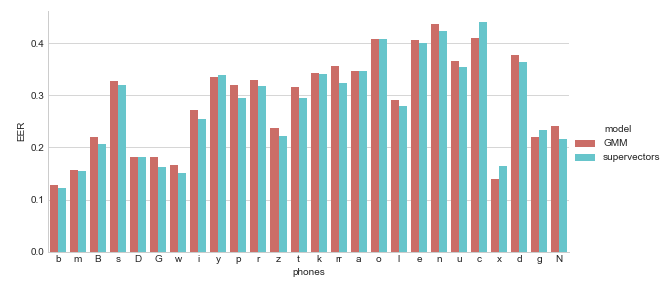
\includegraphics[width=0.8\textwidth]{files/figures/results/gmm-vs-supervectors/gmm-vs-supervectors-dev.png}
	\caption{Comparison of EER between LLR from Adapted GMMs with K-Means initialization
	and SVM trained on Supervectors for all phones in the training set, sorted
	descendently by Kappa values.}
	\label{fig:gmmSupervectorsDev}
\end{figure}

\begin{figure}[H]
	\centering
	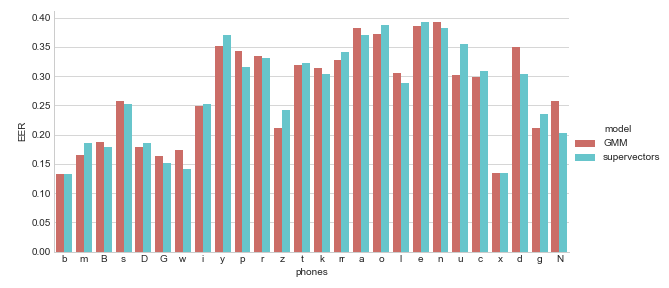
\includegraphics[width=0.8\textwidth]{files/figures/results/gmm-vs-supervectors/gmm-vs-supervectors-heldout.png}
	\caption{Comparison of EER between LLR from Adapted GMMs with K-Means initialization
	and SVM trained on Supervectors for all phones in the test set, sorted descendently
	by Kappa values.}
	\label{fig:gmmSupervectorsTest}
\end{figure}


\section{Legendre Best System}

\begin{figure}[H]
	\centering
	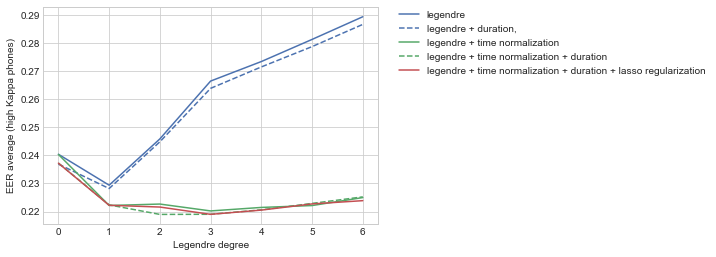
\includegraphics[width=1.0\textwidth]{files/figures/results/legendre-dct/legendre-tunning.png}
	\caption{EER average over phonemes with high Kappa for different 
	degrees of Legendre Polynomials in
	the training set. Additional configurations are also studied along with the degree and 
	represented by different curves: time normalization, appending the duration and applying
	Lasso Regression}
	\label{fig:legendreTunning}
\end{figure}


\section{Legendre vs DCT}

\begin{figure}[H]
	\centering
	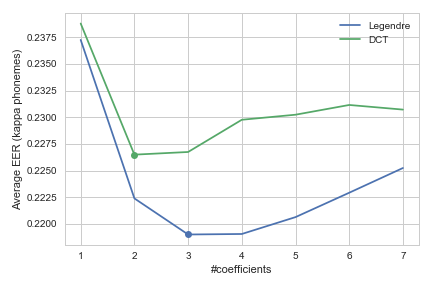
\includegraphics[width=0.5\textwidth]{files/figures/results/legendre-dct/legendre-dct-coefficients.png}
	\caption{EER average over phonemes with high Kappa as function of the number of coefficients
	for both Legendre Polynomials and DCT in the training set.}
	\label{fig:legendreVsDCT}
\end{figure}


\section{Fusion systems}

\subsection{Statistical Significant Filtering}

\subsection{Plots}

\begin{figure}[H]
	\centering
	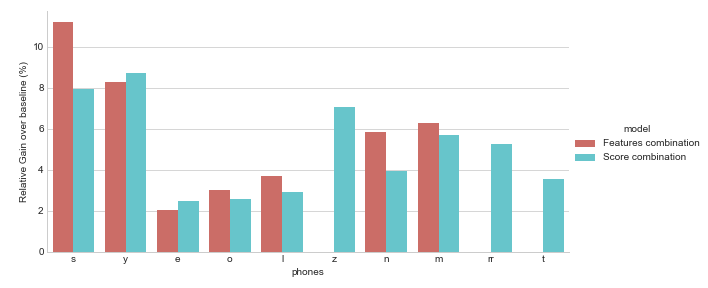
\includegraphics[width=0.8\textwidth]{files/figures/results/relatives/relatives-fusion-systems-dev-mcnemar.png}
	\caption{Comparison of performance between Features Combination system and the score combination
	of individual systems in the training set for the phones whose results were significant 
	in the training set, sorted descendently by their p-value obtained in the McNemar test. 
	For all the score combinations phones the results were significant in the training set,
	whereas for the features combination phones only the phones marked with (*) were significant, 
	and those marked with (**) weren't significant.}
	\label{fig:fusionMcnemarDev}
\end{figure}

\begin{figure}[H]
	\centering
	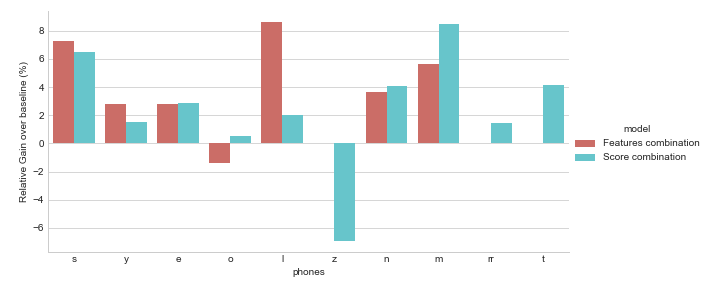
\includegraphics[width=0.8\textwidth]{files/figures/results/relatives/relative-fusion-systems-heldout-mcnemar.png}
	\caption{Comparison of performance between Features Combination system and the score combination
	of individual systems in the test set for the phones whose results were significant 
	in the training set, sorted descendently by their p-value obtained in the McNemar test. 
	For all the score combinations phones the results were significant in the training set,
	whereas for the features combination phones only the phones marked with (*) were significant, 
	and those marked with (**) weren't significant.}
	\label{fig:fusionMcnemarTest}
\end{figure}
